\subsubsection{UC5 - Login manuale}
\begin{figure}[H]
	\centering
	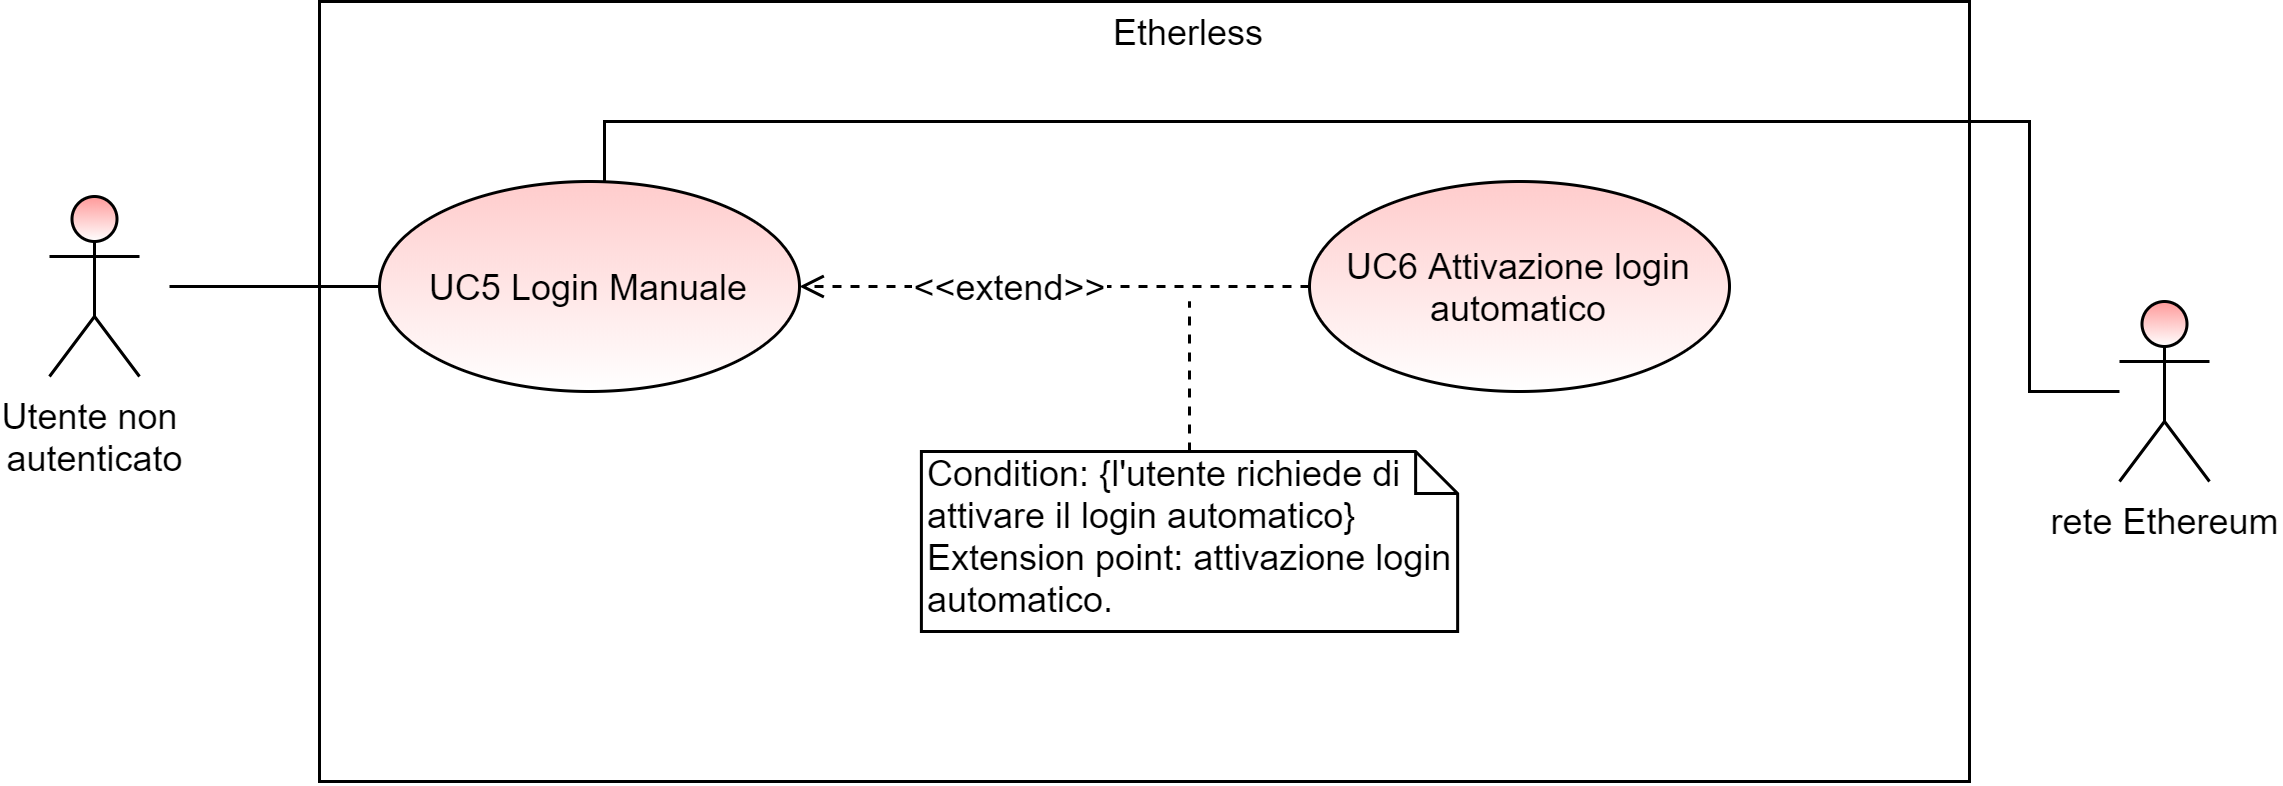
\includegraphics[scale=\ucs]{./res/img/UC5G.png}
	\caption {UC5 - Login manuale: schema generale}
\end{figure}
\begin{figure}[H]
	\centering
	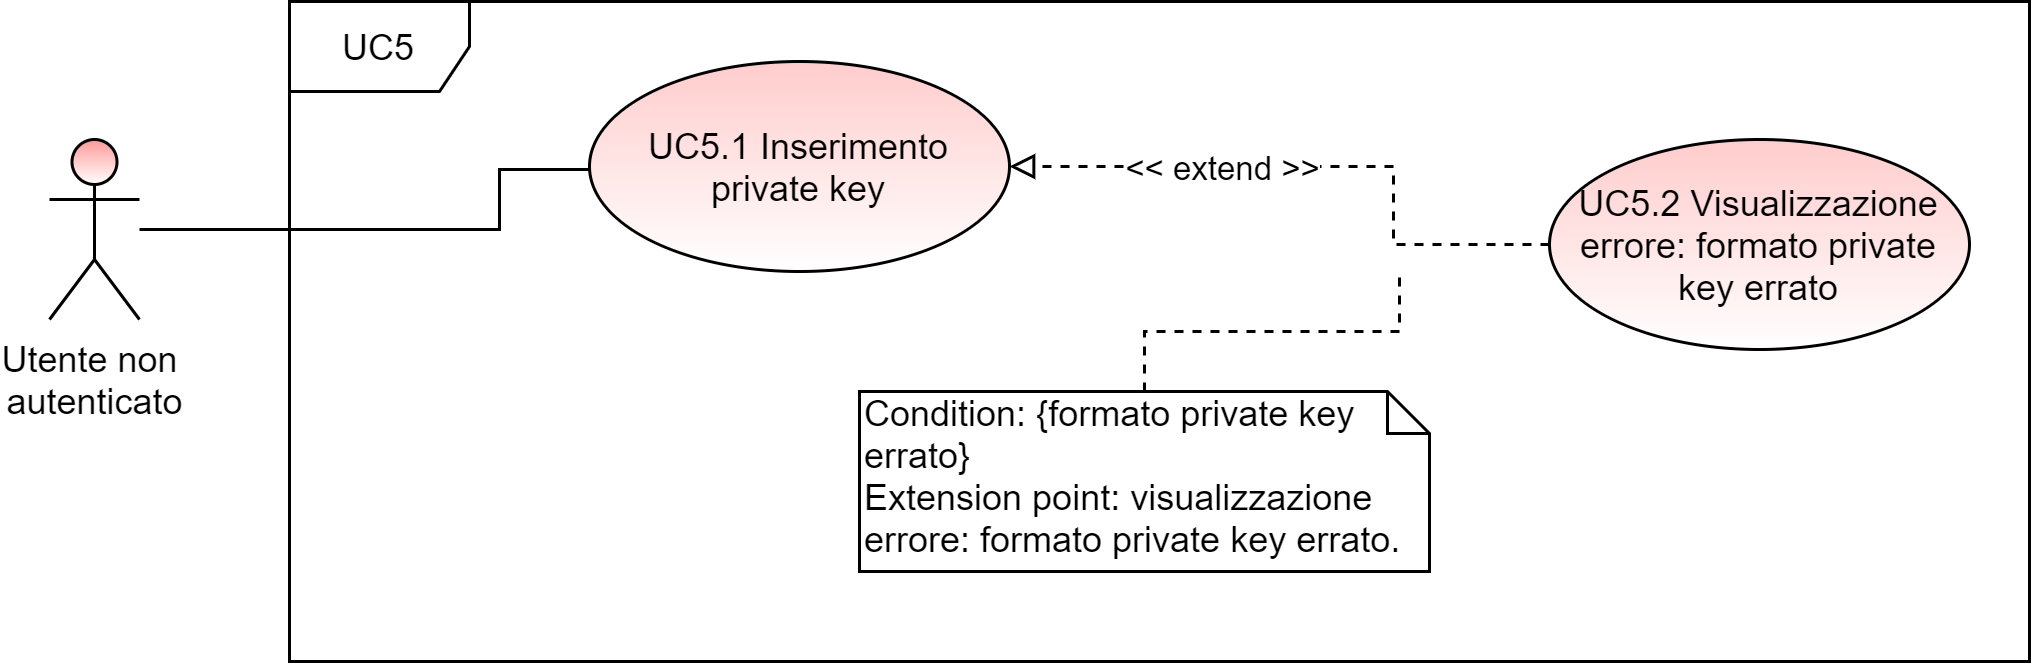
\includegraphics[scale=\ucs]{./res/img/UC5.png}
	\caption {UC5 - Login manuale}
\end{figure}
\begin{itemize}
	\item \textbf{Attori primari:} \una{};
	\item \textbf{Attori secondari:} \re{};
	\item \textbf{Descrizione:} l’utente può utilizzare il comando \login{} per autenticarsi all’interno della rete Ethereum\ped{\textit{G}}; 
	\item \textbf{Scenario principale:} l'utente esegue il comando \login{} indicando manualmente le credenziali necessarie; 
	\item \textbf{Estensioni:} 
	\begin{itemize}
		\item \textbf{UC6:} tramite l’apposito flag \texttt{-r} l’utente può richiedere che le credenziali inserite, se corrette, vengano memorizzate e usate per l'autenticazione automatica in caso di accessi futuri;
	\end{itemize}
	\item \textbf{Precondizione:} l’utente tenta di autenticarsi alla piattaforma;
	\item \textbf{Postcondizione:} l’utente si è autenticato correttamente.
\end{itemize}